Several MVA methods implemented in the TMVA package~\cite{TMVA2007} has been tested and BDTG has been found as
the one that gives the best performance and it is used for this study.
Samples used are HWW with \mHi=120 \GeVcc for signal and a combination of Powheg and Madgraph DY samples for background,
where, for signal, a low mass Higgs sample has been chosen since DY is mostly relevant for low Higgs mass analyses and,
for background, all the available samples have been combined to maximise the statistcs.

The training sample is selected applying cuts as close as possible to the final selection where the MVA selection is applied: 
same flavor final state, full lepton selection with $p_T$$>$20(10) \GeVc\ for the leading (trailing) lepton, 
top veto, extra lepton veto, Z veto, $p_T(\Lep\Lep)$$>$45 \GeVc, min(proj-pfMet, proj-trackMet)$>$20 \GeVc.
The training is performed in the 0- and 1-jet bin separately.

The list of variables used in the training is the following:
\begin{itemize}
\item missing energy variables
\begin{itemize}
\item proj-pfMet
\item proj-trackMet
\item pfMet divided by $\Sigma E_T$: met/$\sqrt{sumet}$;
\end{itemize}
\item kinematic variables
\begin{itemize}
\item dilepton $p_T$: $p_T(\Lep\Lep)$;
\item transverse Higgs mass: $m_T$;
\item leading jet $p_T$: $p_T$(j1);
\item recoil $\equiv$ magnitude of the vector sum of pfMet and dilepton system in the transverse plane;
\end{itemize}
\item azimuthal angles differences
\begin{itemize}
\item between dilepton system and leading jet: $\Delta\phi$($\Lep\Lep$,j1);
\item between dilepton system and pfMet: $\Delta\phi$($\Lep\Lep$,\met);
\item between leading jet and pfMet: $\Delta\phi$(j1,\met);
\end{itemize}
\item other variables
\begin{itemize}
\item number of primary vertices: nvtx.
\end{itemize}
\end{itemize}

Most variables give a good discimination between signal and background (Figures~\ref{fig:TMVAvar_0j} and \ref{fig:TMVAvar_1j}), while others, like nvtx, 
are useful for correlations (Figures~\ref{fig:lincorr0j} and \ref{fig:lincorr1j}).
The resulting output distributions show a very large separation of the signal from the background and no evidence of 
over-training (Figures~\ref{fig:mvaout_jae_0j_log} and \ref{fig:mvaout_jae_1j_log}).
This variable will be called DY MVA in the rest of this note.

Given that the training is performed on MC samples, it is crucial that the input variables are well reproduced by data.
Figures~\ref{fig:pmet}-\ref{fig:nvtx} show the variables in data after the training selection.
Events requiring a Z mass veto, corresponding to the actual training sample, are more contaminated by backgrounds, while events under the Z peak are dominated by DY.
Flavor-symmetric backgrounds (\W\W\ and Top) are taken from opposite flavor data properly weighted for the e-$\mu$ selection efficiency difference, while \W\Z\ 
and \Z\Z\ backgrounds are taken from MC. For visualization purposed, the DY contribution is scaled by an ad-hoc factor to match the bulk of the events in data.
In all cases, MC reproduces with reasonable accuracy the features observed in data.

%%%%%%%%
\begin{figure}[!hbtp]
\begin{center}
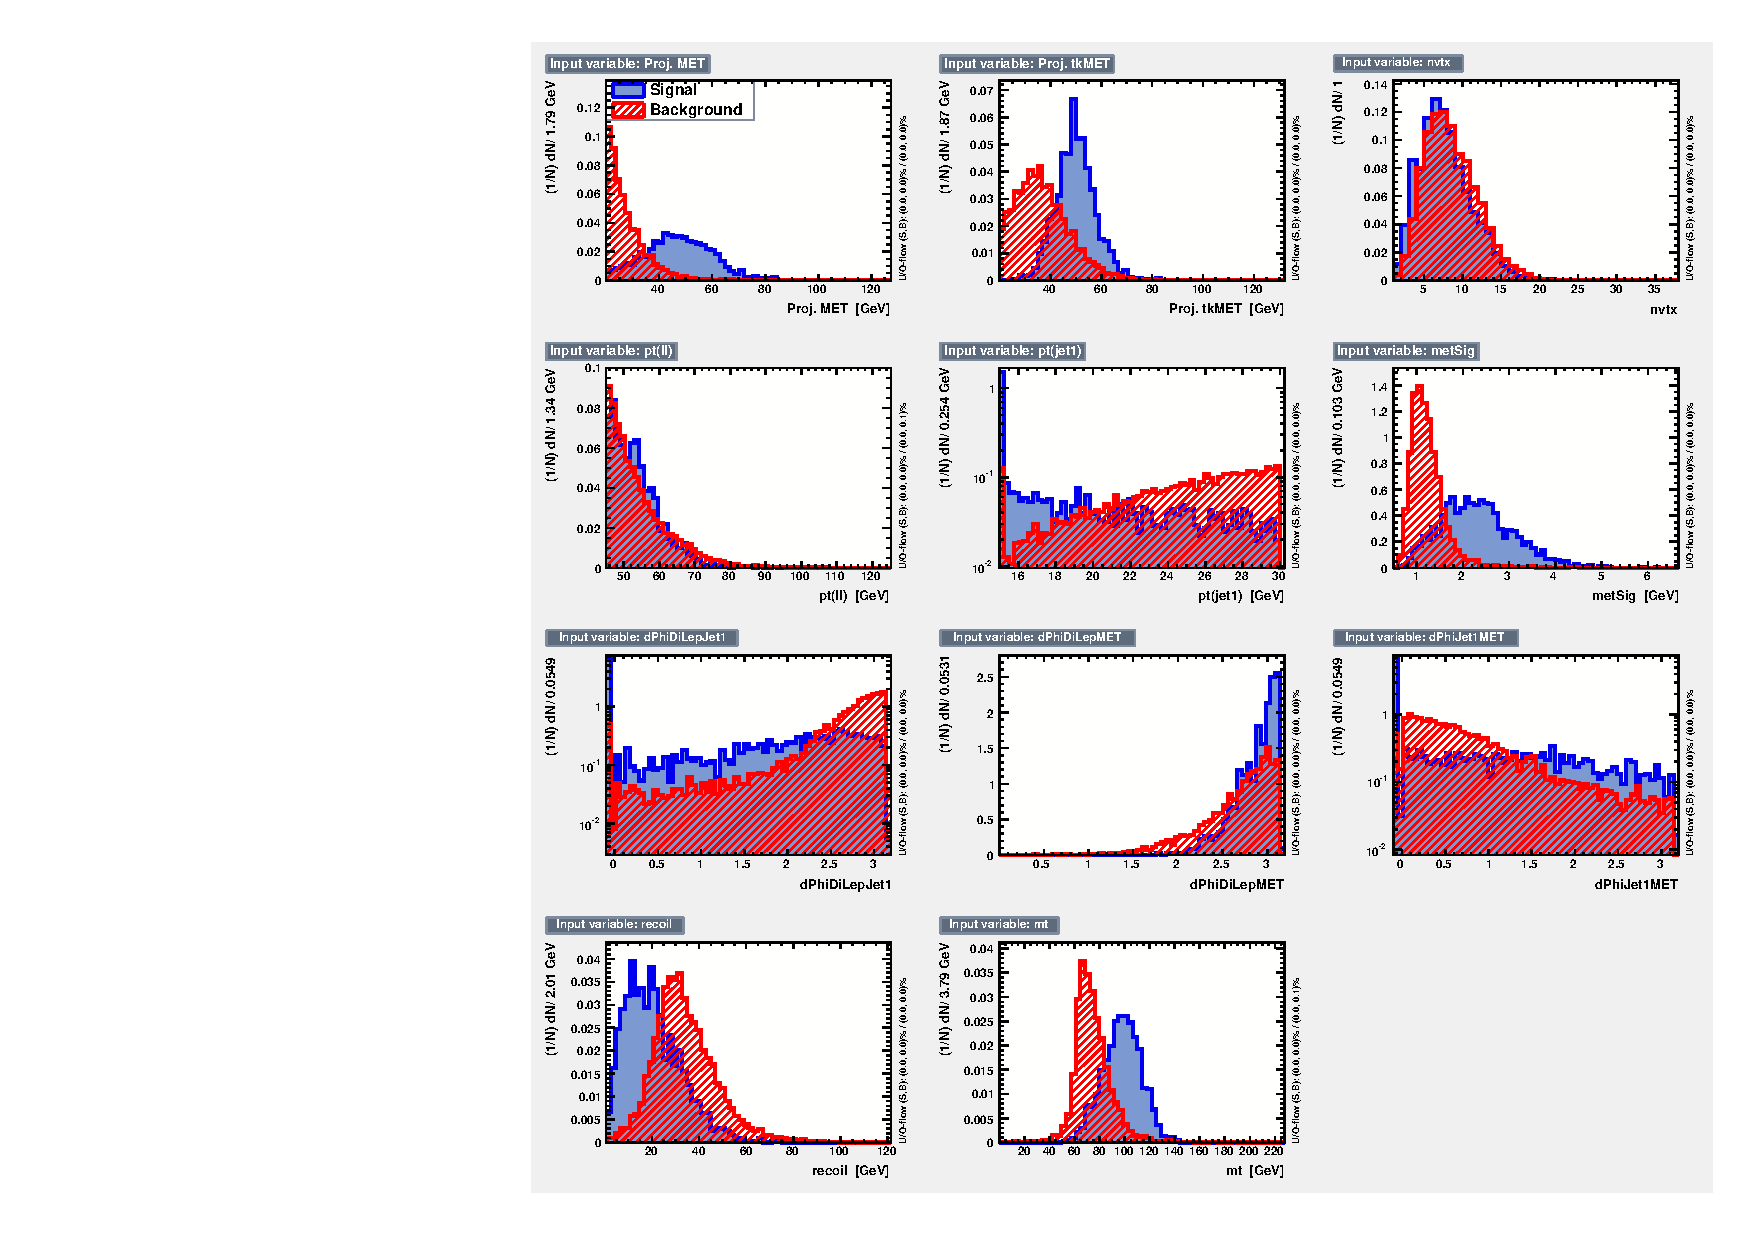
\includegraphics[width=.9\textwidth]{figures/TMVAvar_0j.pdf}
\caption{Input training variables for 0-jet bin.}
\label{fig:TMVAvar_0j}
\end{center}
\end{figure}
%%%%%%%%

%%%%%%%%
\begin{figure}[!hbtp]
\begin{center}
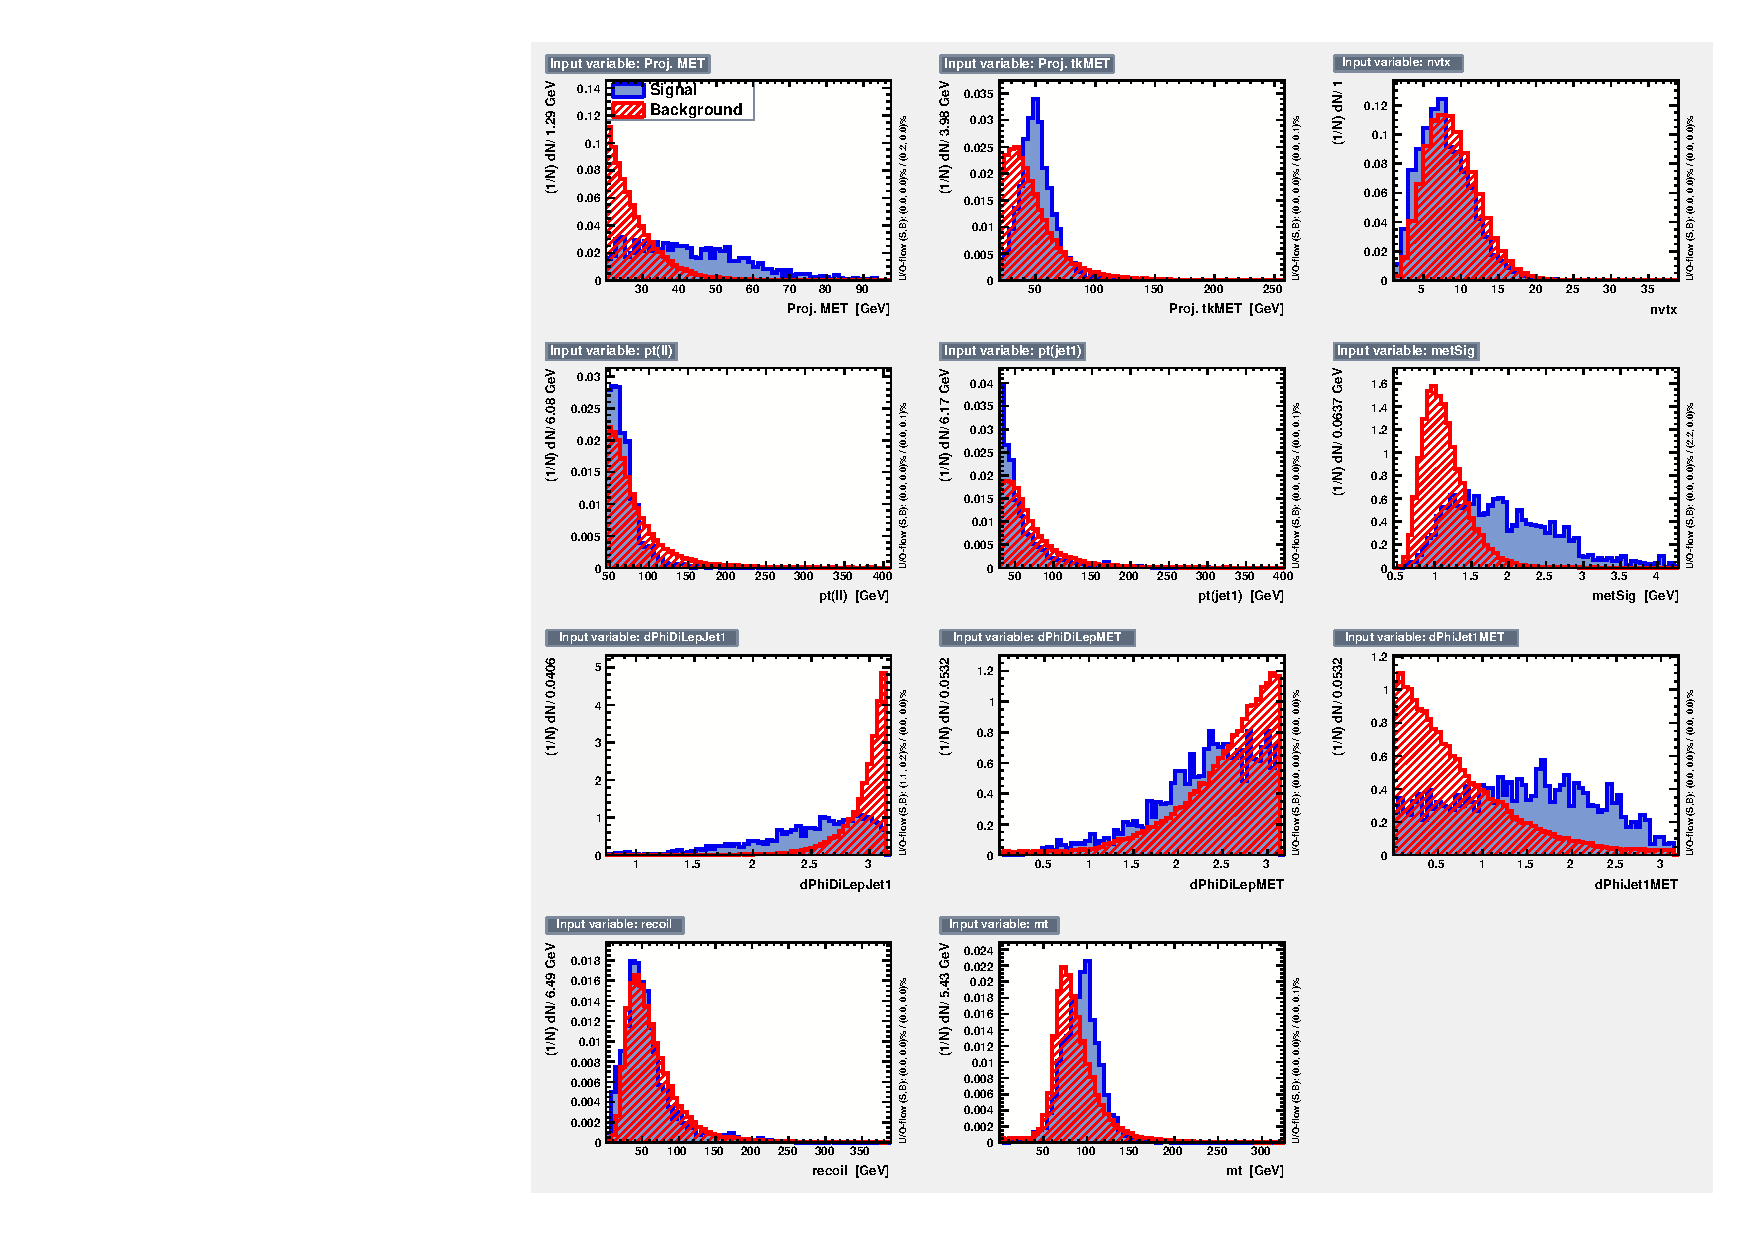
\includegraphics[width=.9\textwidth]{figures/TMVAvar_1j.pdf}
\caption{Input training variables for 1-jet bin.}
\label{fig:TMVAvar_1j}
\end{center}
\end{figure}
%%%%%%%%

%%%%%%%%
\begin{figure}[!hbtp]
\begin{center}
\subfigure[Signal]{\label{subfig:CorrelationMatrixS_0j}
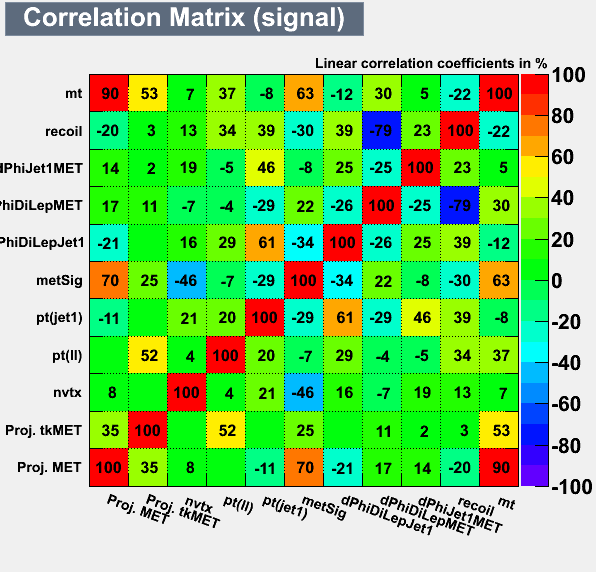
\includegraphics[width=.45\textwidth]{figures/CorrelationMatrixS_0j.png}}
\subfigure[Background]{\label{subfig:CorrelationMatrixB_0j}
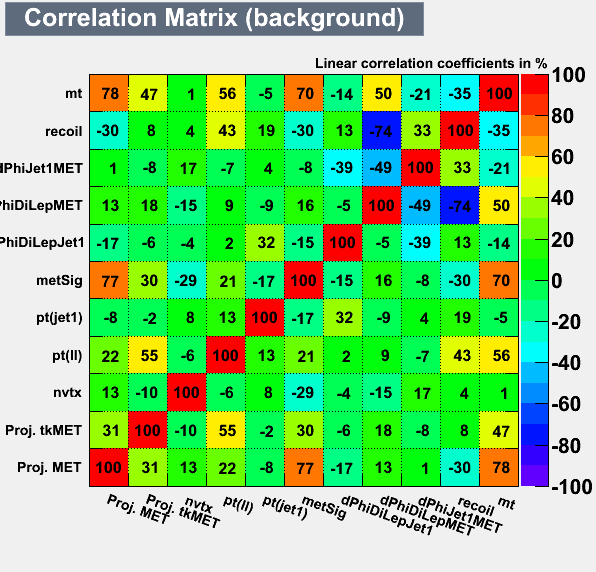
\includegraphics[width=.45\textwidth]{figures/CorrelationMatrixB_0j.png}}
\caption{Linear correlation coefficients (0-jet bin).}
\label{fig:lincorr0j}
\end{center}
\end{figure}
%%%%%%%%

%%%%%%%%
\begin{figure}[!hbtp]
\begin{center}
\subfigure[Signal]{\label{subfig:CorrelationMatrixS_1j}
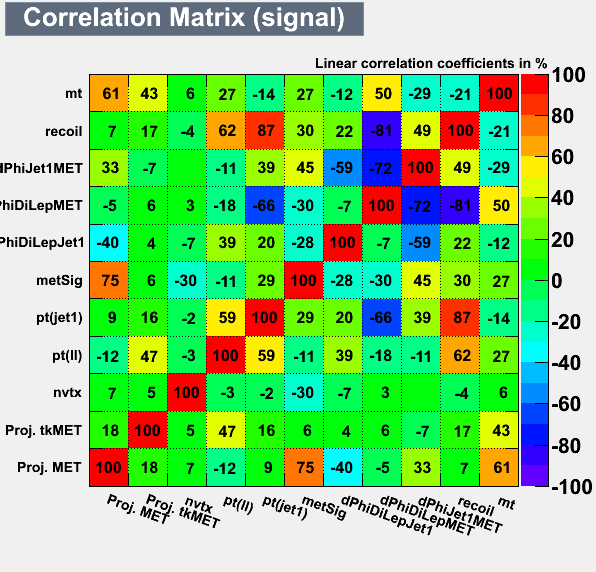
\includegraphics[width=.45\textwidth]{figures/CorrelationMatrixS_1j.png}}
\subfigure[Background]{\label{subfig:CorrelationMatrixB_1j}
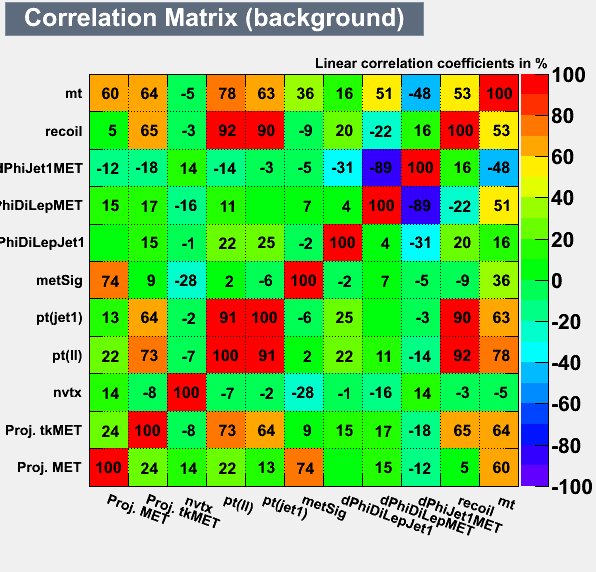
\includegraphics[width=.45\textwidth]{figures/CorrelationMatrixB_1j.png}}
\caption{Linear correlation coefficients (1-jet bin).}
\label{fig:lincorr1j}
\end{center}
\end{figure}
%%%%%%%%

%%%%%%%%
\begin{figure}[!hbtp]
\begin{center}
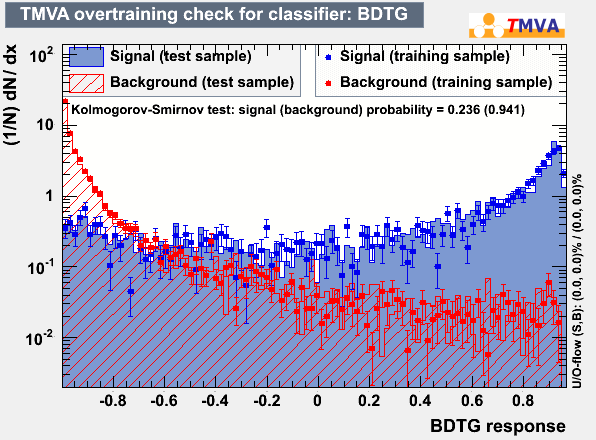
\includegraphics[width=.6\textwidth]{figures/mvaout_jae_0j_log.png}
\caption{MVA output for signal and background, with training and test samples superimposed (0-jet bin).}
\label{fig:mvaout_jae_0j_log}
\end{center}
\end{figure}
%%%%%%%%

%%%%%%%%
\begin{figure}[!hbtp]
\begin{center}
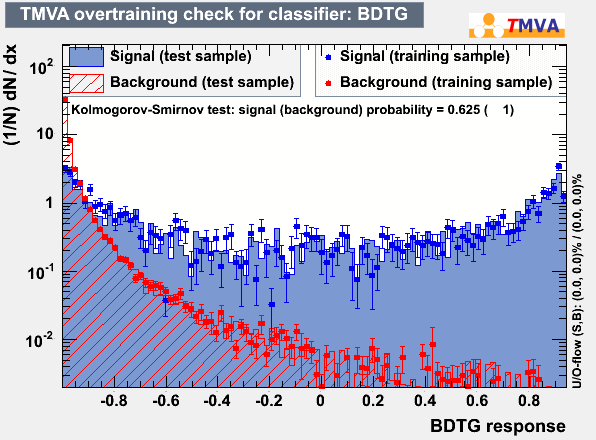
\includegraphics[width=.6\textwidth]{figures/mvaout_jae_1j_log.png}
\caption{MVA output for signal and background, with training and test samples superimposed (1-jet bin).}
\label{fig:mvaout_jae_1j_log}
\end{center}
\end{figure}
%%%%%%%%

%%%%%%%%
\begin{figure}[!hbtp]
\begin{center}
\subfigure[Z peak, 0-jet]{\label{subfig:ZpMet20ptll45_0j_ll/pmet_0j}
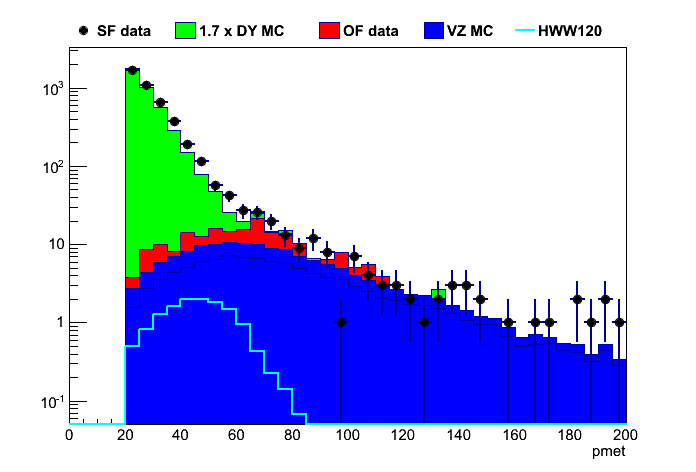
\includegraphics[width=.4\textwidth]{figures/ZpMet20ptll45_0j_ll/pmet_0j.png}}
\subfigure[Z peak, 1-jet]{\label{subfig:ZpMet20ptll45_1j_ll/pmet_1j}
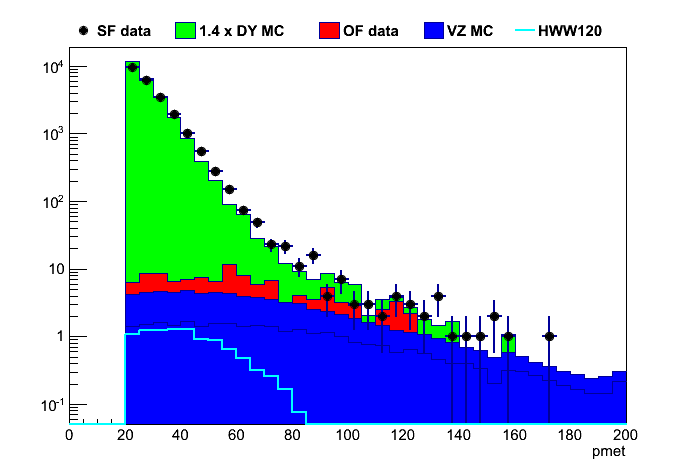
\includegraphics[width=.4\textwidth]{figures/ZpMet20ptll45_1j_ll/pmet_1j.png}}\\
\subfigure[Z veto, 0-jet]{\label{subfig:oZMet20ptll45_0j_ll/pmet_0j}
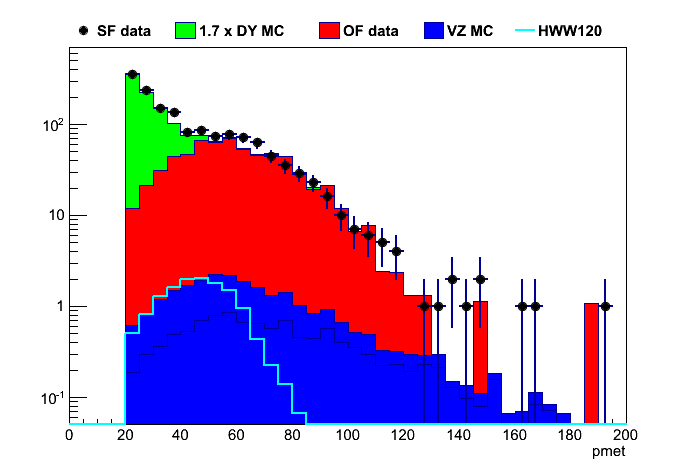
\includegraphics[width=.4\textwidth]{figures/oZMet20ptll45_0j_ll/pmet_0j.png}}
\subfigure[Z veto, 1-jet]{\label{subfig:oZMet20ptll45_1j_ll/pmet_1j}
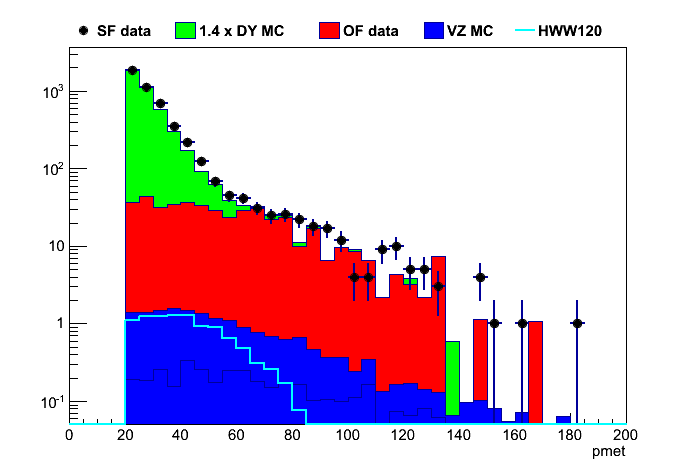
\includegraphics[width=.4\textwidth]{figures/oZMet20ptll45_1j_ll/pmet_1j.png}}
\caption{proj-pfMet distribution in data and MC for 0- and 1-jet bin, where
Z veto $\equiv$ $|$\mll-$m_Z$$|$$>$15~\GeVcc and Z peak $\equiv$ $|$\mll-$m_Z$$|$$<$7.5~\GeVcc.}
\label{fig:pmet}
\end{center}
\end{figure}
%%%%%%%%

%%%%%%%%
\begin{figure}[!hbtp]
\begin{center}
\subfigure[Z peak, 0-jet]{\label{subfig:ZpMet20ptll45_0j_ll/pTrackMet_0j}
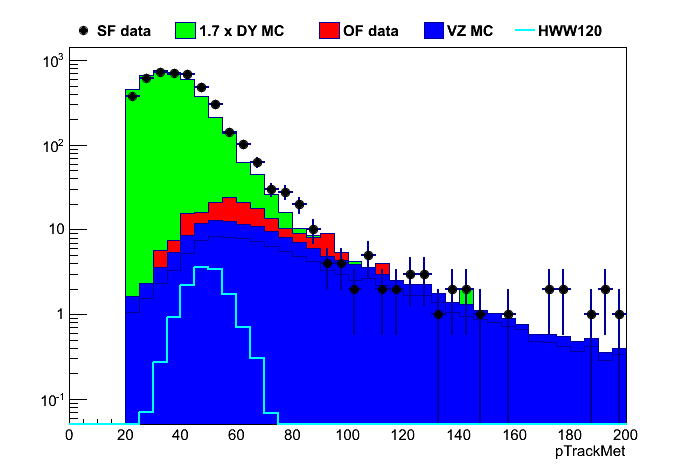
\includegraphics[width=.4\textwidth]{figures/ZpMet20ptll45_0j_ll/pTrackMet_0j.png}}
\subfigure[Z peak, 1-jet]{\label{subfig:ZpMet20ptll45_1j_ll/pTrackMet_1j}
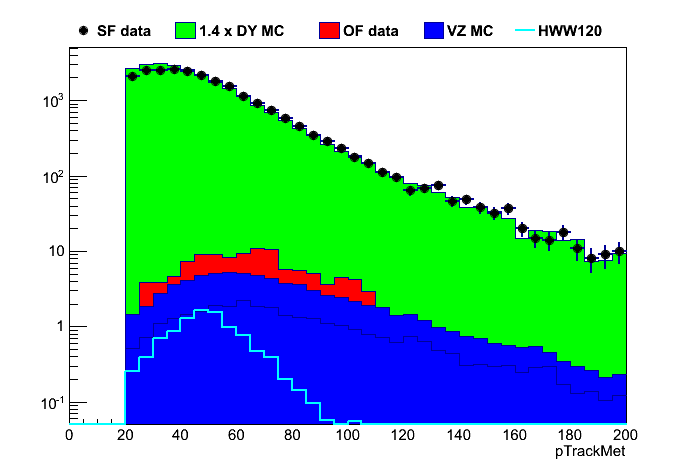
\includegraphics[width=.4\textwidth]{figures/ZpMet20ptll45_1j_ll/pTrackMet_1j.png}}\\
\subfigure[Z veto, 0-jet]{\label{subfig:oZMet20ptll45_0j_ll/pTrackMet_0j}
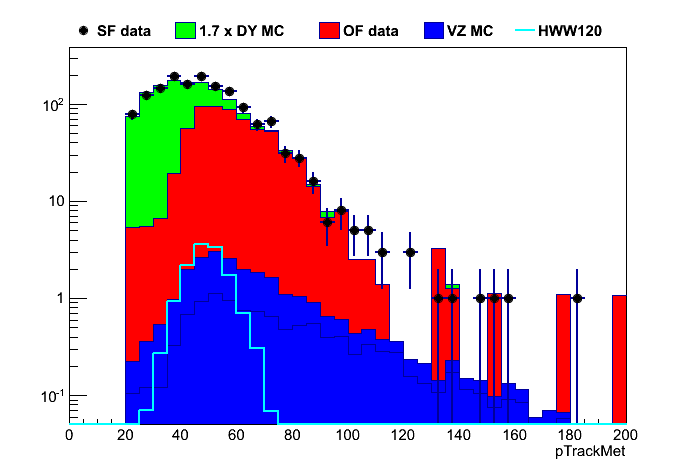
\includegraphics[width=.4\textwidth]{figures/oZMet20ptll45_0j_ll/pTrackMet_0j.png}}
\subfigure[Z veto, 1-jet]{\label{subfig:oZMet20ptll45_1j_ll/pTrackMet_1j}
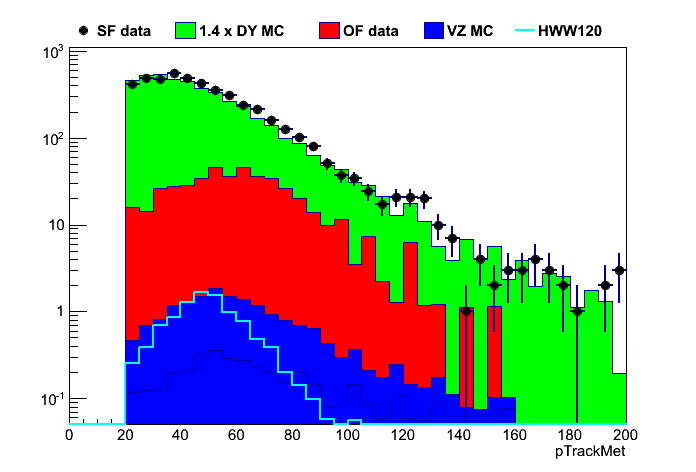
\includegraphics[width=.4\textwidth]{figures/oZMet20ptll45_1j_ll/pTrackMet_1j.png}}
\caption{proj-trackMet distribution in data and MC for 0- and 1-jet bin, where
Z veto $\equiv$ $|$\mll-$m_Z$$|$$>$15~\GeVcc and Z peak $\equiv$ $|$\mll-$m_Z$$|$$<$7.5~\GeVcc.}
\label{fig:pTrackMet}
\end{center}
\end{figure}
%%%%%%%%

%%%%%%%%
\begin{figure}[!hbtp]
\begin{center}
\subfigure[Z peak, 0-jet]{\label{subfig:ZpMet20ptll45_0j_ll/metsqrtsumet_0j}
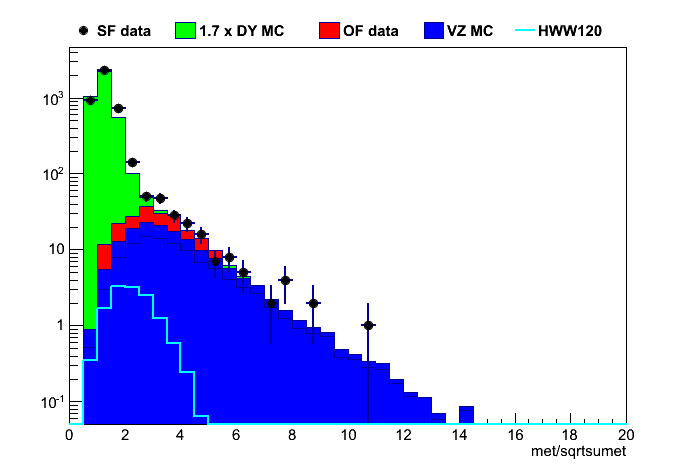
\includegraphics[width=.4\textwidth]{figures/ZpMet20ptll45_0j_ll/metsqrtsumet_0j.png}}
\subfigure[Z peak, 1-jet]{\label{subfig:ZpMet20ptll45_1j_ll/metsqrtsumet_1j}
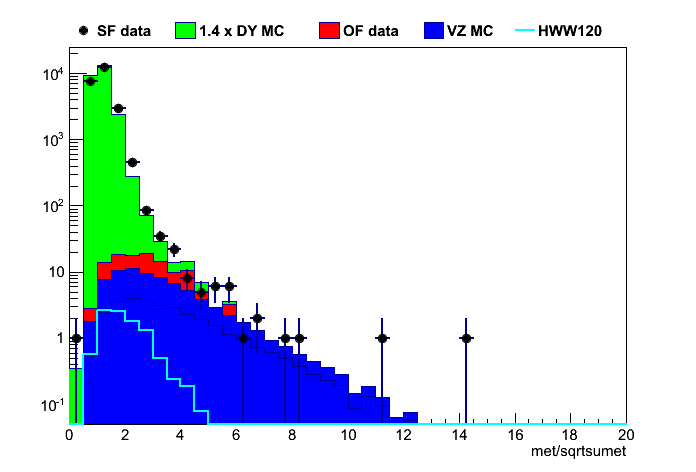
\includegraphics[width=.4\textwidth]{figures/ZpMet20ptll45_1j_ll/metsqrtsumet_1j.png}}\\
\subfigure[Z veto, 0-jet]{\label{subfig:oZMet20ptll45_0j_ll/metsqrtsumet_0j}
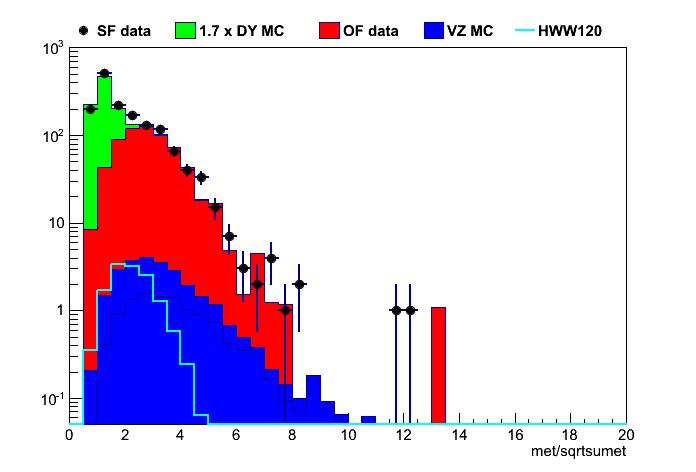
\includegraphics[width=.4\textwidth]{figures/oZMet20ptll45_0j_ll/metsqrtsumet_0j.png}}
\subfigure[Z veto, 1-jet]{\label{subfig:oZMet20ptll45_1j_ll/metsqrtsumet_1j}
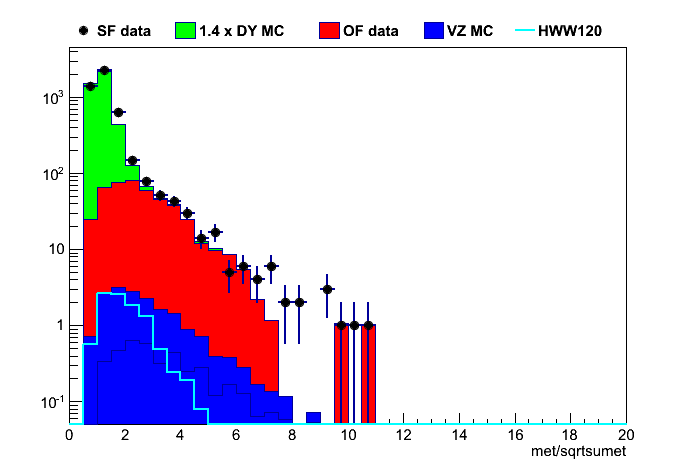
\includegraphics[width=.4\textwidth]{figures/oZMet20ptll45_1j_ll/metsqrtsumet_1j.png}}
\caption{met/$\sqrt{sumet}$ distribution in data and MC for 0- and 1-jet bin, where
Z veto $\equiv$ $|$\mll-$m_Z$$|$$>$15~\GeVcc and Z peak $\equiv$ $|$\mll-$m_Z$$|$$<$7.5~\GeVcc.}
\label{fig:metsqrtsumet}
\end{center}
\end{figure}
%%%%%%%%

%%%%%%%%
\begin{figure}[!hbtp]
\begin{center}
\subfigure[Z peak, 0-jet]{\label{subfig:ZpMet20ptll45_0j_ll/dileppt_0j}
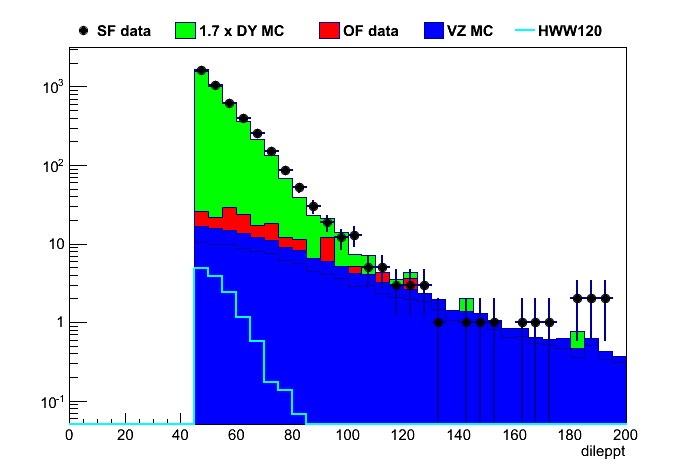
\includegraphics[width=.4\textwidth]{figures/ZpMet20ptll45_0j_ll/dileppt_0j.png}}
\subfigure[Z peak, 1-jet]{\label{subfig:ZpMet20ptll45_1j_ll/dileppt_1j}
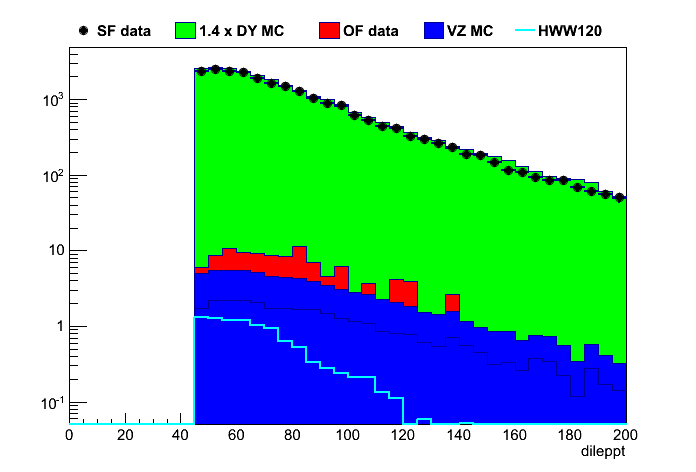
\includegraphics[width=.4\textwidth]{figures/ZpMet20ptll45_1j_ll/dileppt_1j.png}}\\
\subfigure[Z veto, 0-jet]{\label{subfig:oZMet20ptll45_0j_ll/dileppt_0j}
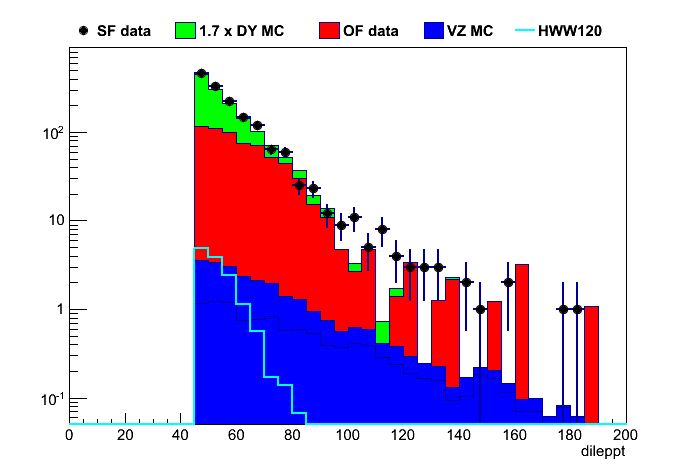
\includegraphics[width=.4\textwidth]{figures/oZMet20ptll45_0j_ll/dileppt_0j.png}}
\subfigure[Z veto, 1-jet]{\label{subfig:oZMet20ptll45_1j_ll/dileppt_1j}
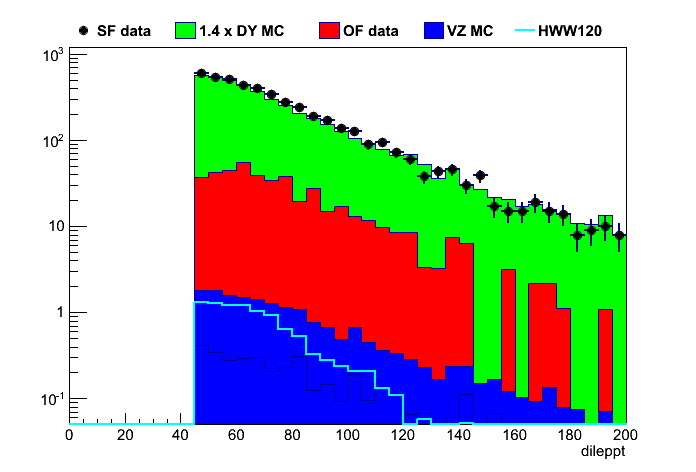
\includegraphics[width=.4\textwidth]{figures/oZMet20ptll45_1j_ll/dileppt_1j.png}}
\caption{Dileption $p_T$ distribution in data and MC for 0- and 1-jet bin, where
Z veto $\equiv$ $|$\mll-$m_Z$$|$$>$15~\GeVcc and Z peak $\equiv$ $|$\mll-$m_Z$$|$$<$7.5~\GeVcc.}
\label{fig:dileppt}
\end{center}
\end{figure}
%%%%%%%%

%%%%%%%%
\begin{figure}[!hbtp]
\begin{center}
\subfigure[Z peak, 0-jet]{\label{subfig:ZpMet20ptll45_0j_ll/mt_0j}
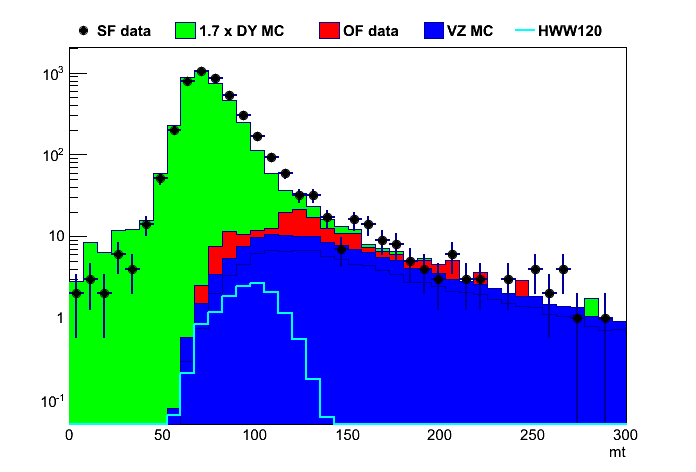
\includegraphics[width=.4\textwidth]{figures/ZpMet20ptll45_0j_ll/mt_0j.png}}
\subfigure[Z peak, 1-jet]{\label{subfig:ZpMet20ptll45_1j_ll/mt_1j}
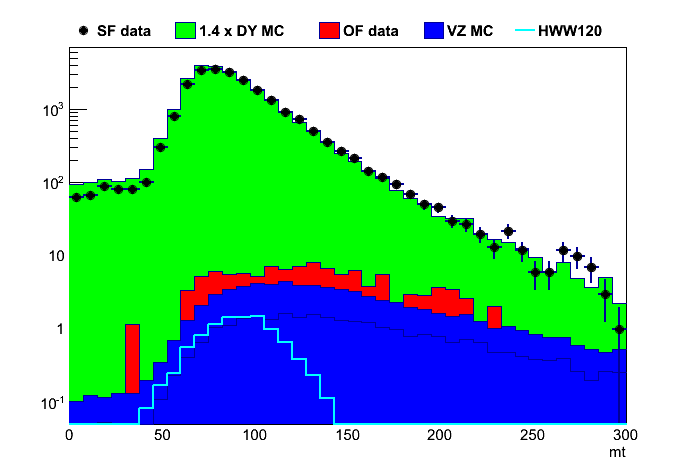
\includegraphics[width=.4\textwidth]{figures/ZpMet20ptll45_1j_ll/mt_1j.png}}\\
\subfigure[Z veto, 0-jet]{\label{subfig:oZMet20ptll45_0j_ll/mt_0j}
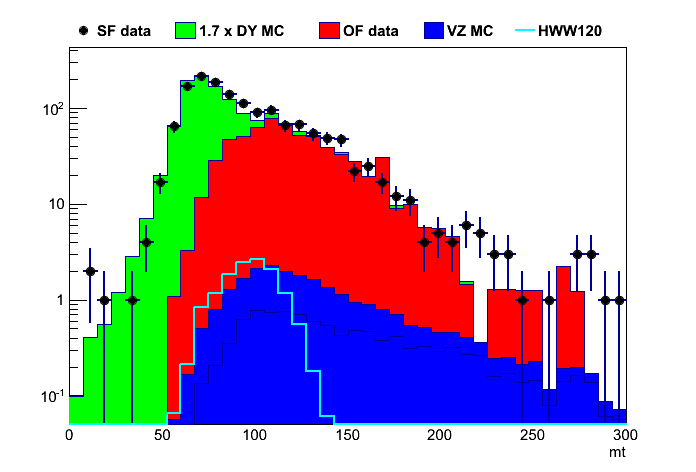
\includegraphics[width=.4\textwidth]{figures/oZMet20ptll45_0j_ll/mt_0j.png}}
\subfigure[Z veto, 1-jet]{\label{subfig:oZMet20ptll45_1j_ll/mt_1j}
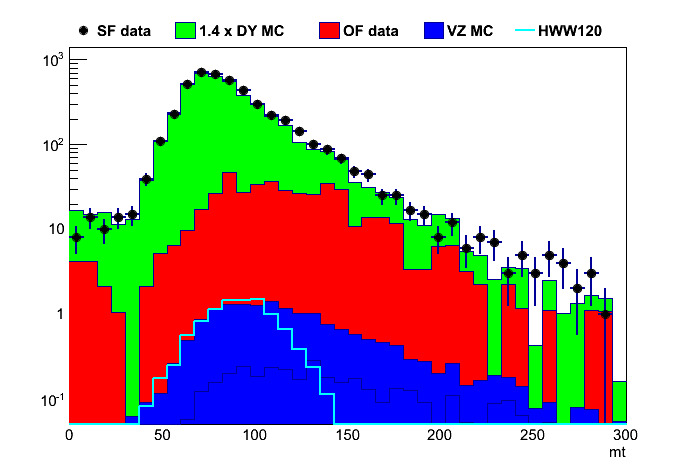
\includegraphics[width=.4\textwidth]{figures/oZMet20ptll45_1j_ll/mt_1j.png}}
\caption{$m_T$ distribution in data and MC for 0- and 1-jet bin, where
Z veto $\equiv$ $|$\mll-$m_Z$$|$$>$15~\GeVcc and Z peak $\equiv$ $|$\mll-$m_Z$$|$$<$7.5~\GeVcc.}
\label{fig:mt}
\end{center}
\end{figure}
%%%%%%%%

%%%%%%%%
\begin{figure}[!hbtp]
\begin{center}
\subfigure[Z peak, 0-jet]{\label{subfig:ZpMet20ptll45_0j_ll/jet1pt_0j}
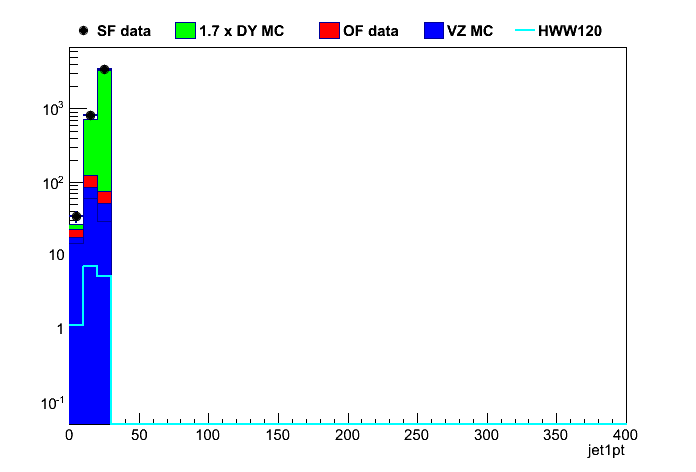
\includegraphics[width=.4\textwidth]{figures/ZpMet20ptll45_0j_ll/jet1pt_0j.png}}
\subfigure[Z peak, 1-jet]{\label{subfig:ZpMet20ptll45_1j_ll/jet1pt_1j}
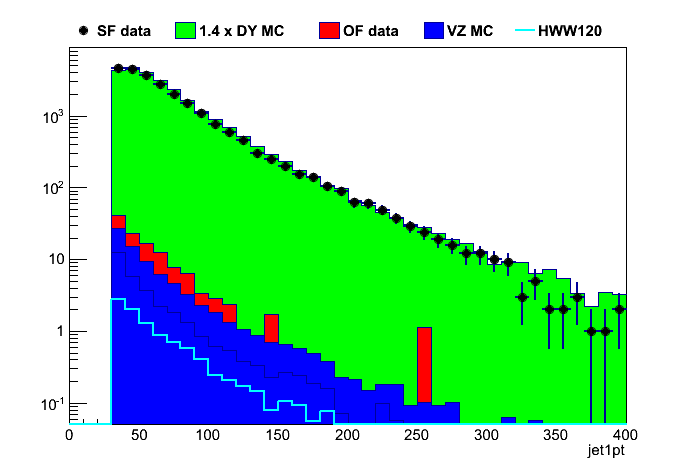
\includegraphics[width=.4\textwidth]{figures/ZpMet20ptll45_1j_ll/jet1pt_1j.png}}\\
\subfigure[Z veto, 0-jet]{\label{subfig:oZMet20ptll45_0j_ll/jet1pt_0j}
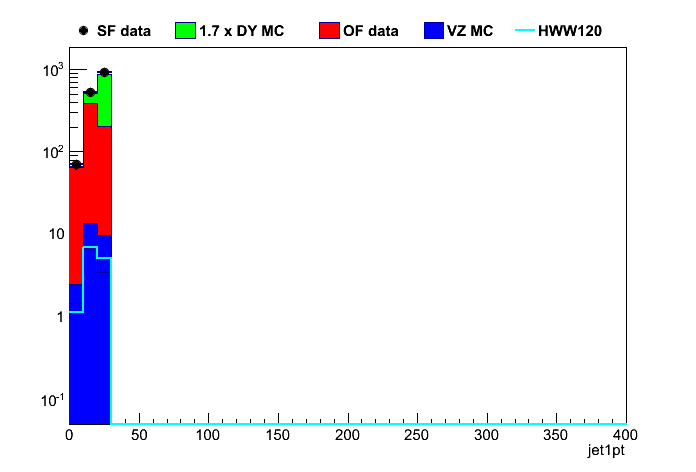
\includegraphics[width=.4\textwidth]{figures/oZMet20ptll45_0j_ll/jet1pt_0j.png}}
\subfigure[Z veto, 1-jet]{\label{subfig:oZMet20ptll45_1j_ll/jet1pt_1j}
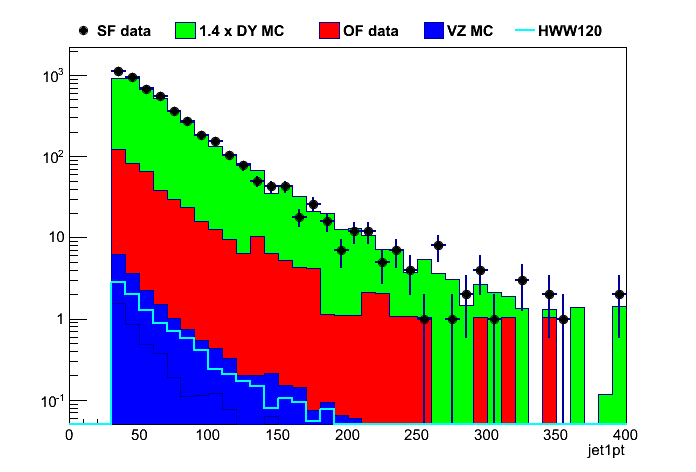
\includegraphics[width=.4\textwidth]{figures/oZMet20ptll45_1j_ll/jet1pt_1j.png}}
\caption{Leading jet $p_T$ distribution in data and MC for 0- and 1-jet bin, where
Z veto $\equiv$ $|$\mll-$m_Z$$|$$>$15~\GeVcc and Z peak $\equiv$ $|$\mll-$m_Z$$|$$<$7.5~\GeVcc.}
\label{fig:jet1pt}
\end{center}
\end{figure}
%%%%%%%%


%%%%%%%%
\begin{figure}[!hbtp]
\begin{center}
\subfigure[Z peak, 0-jet]{\label{subfig:ZpMet20ptll45_0j_ll/recoil_0j}
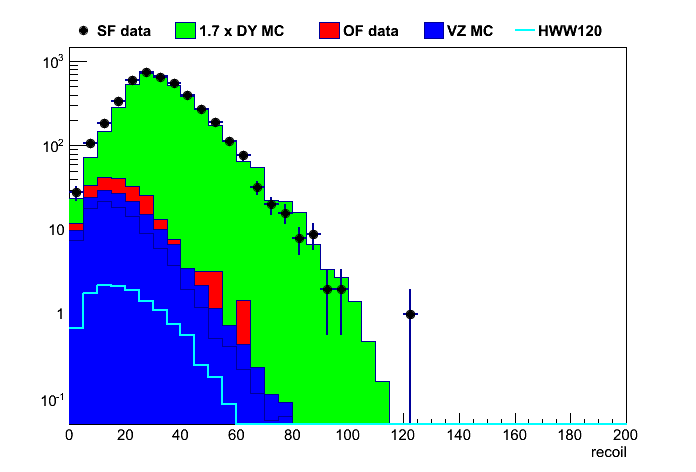
\includegraphics[width=.4\textwidth]{figures/ZpMet20ptll45_0j_ll/recoil_0j.png}}
\subfigure[Z peak, 1-jet]{\label{subfig:ZpMet20ptll45_1j_ll/recoil_1j}
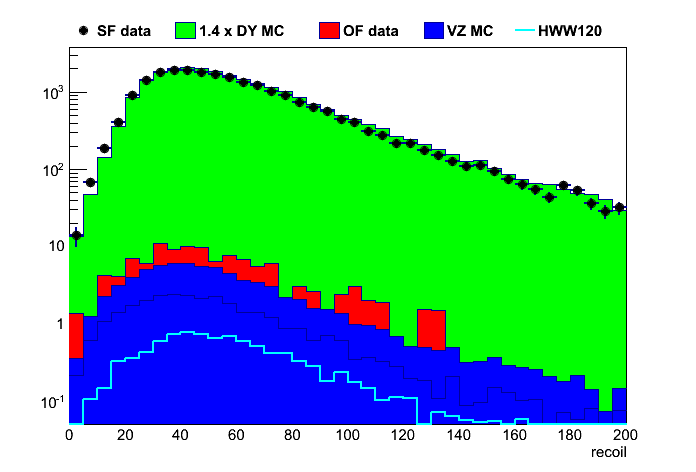
\includegraphics[width=.4\textwidth]{figures/ZpMet20ptll45_1j_ll/recoil_1j.png}}\\
\subfigure[Z veto, 0-jet]{\label{subfig:oZMet20ptll45_0j_ll/recoil_0j}
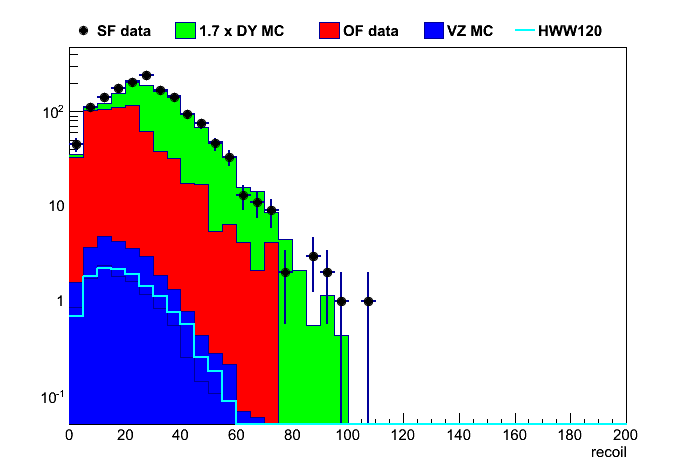
\includegraphics[width=.4\textwidth]{figures/oZMet20ptll45_0j_ll/recoil_0j.png}}
\subfigure[Z veto, 1-jet]{\label{subfig:oZMet20ptll45_1j_ll/recoil_1j}
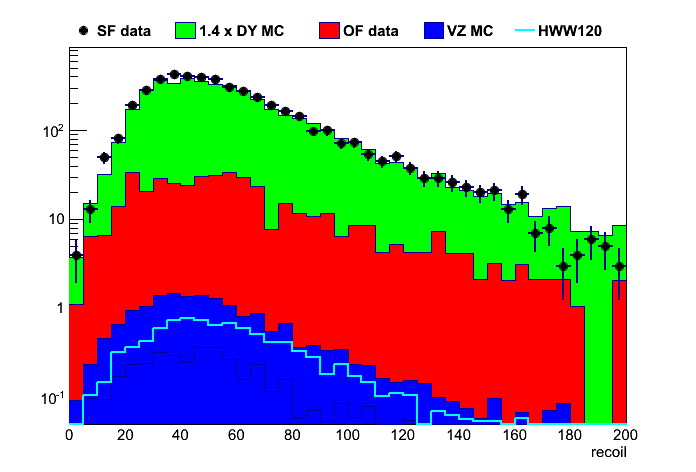
\includegraphics[width=.4\textwidth]{figures/oZMet20ptll45_1j_ll/recoil_1j.png}}
\caption{Recoil variable distribution in data and MC for 0- and 1-jet bin, where
Z veto $\equiv$ $|$\mll-$m_Z$$|$$>$15~\GeVcc and Z peak $\equiv$ $|$\mll-$m_Z$$|$$<$7.5~\GeVcc.}
\label{fig:recoil}
\end{center}
\end{figure}
%%%%%%%%

%%%%%%%%
\begin{figure}[!hbtp]
\begin{center}
\subfigure[Z peak, 0-jet]{\label{subfig:ZpMet20ptll45_0j_ll/dPhiDiLepJet1_0j}
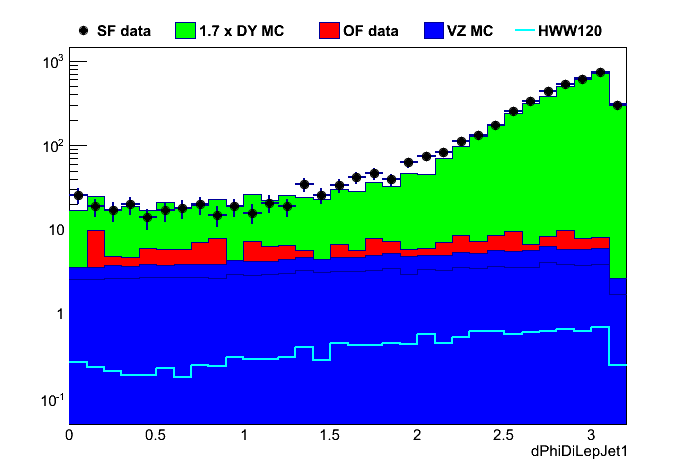
\includegraphics[width=.4\textwidth]{figures/ZpMet20ptll45_0j_ll/dPhiDiLepJet1_0j.png}}
\subfigure[Z peak, 1-jet]{\label{subfig:ZpMet20ptll45_1j_ll/dPhiDiLepJet1_1j}
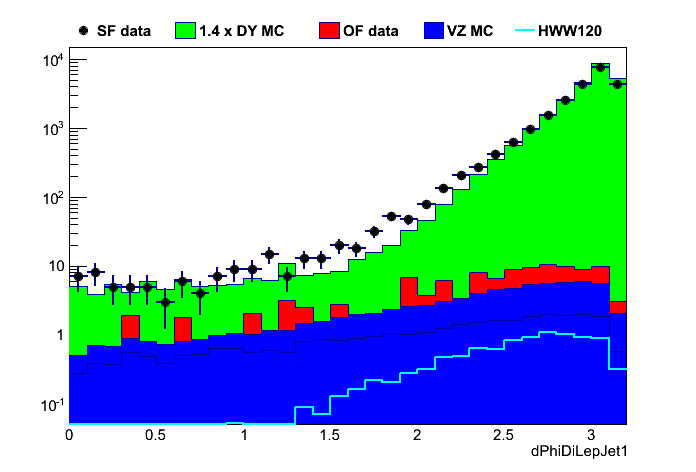
\includegraphics[width=.4\textwidth]{figures/ZpMet20ptll45_1j_ll/dPhiDiLepJet1_1j.png}}\\
\subfigure[Z veto, 0-jet]{\label{subfig:oZMet20ptll45_0j_ll/dPhiDiLepJet1_0j}
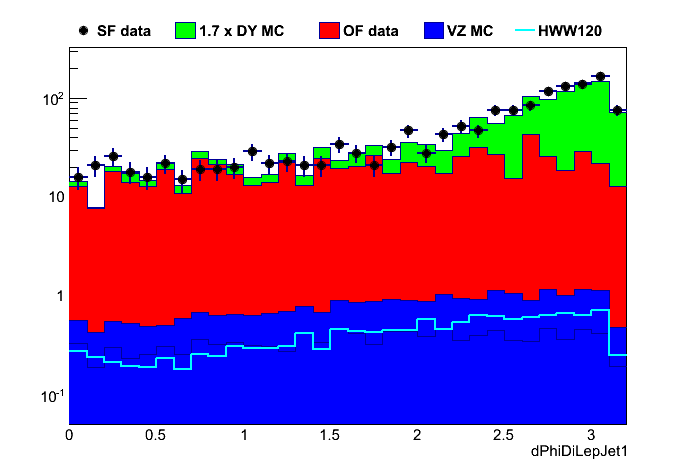
\includegraphics[width=.4\textwidth]{figures/oZMet20ptll45_0j_ll/dPhiDiLepJet1_0j.png}}
\subfigure[Z veto, 1-jet]{\label{subfig:oZMet20ptll45_1j_ll/dPhiDiLepJet1_1j}
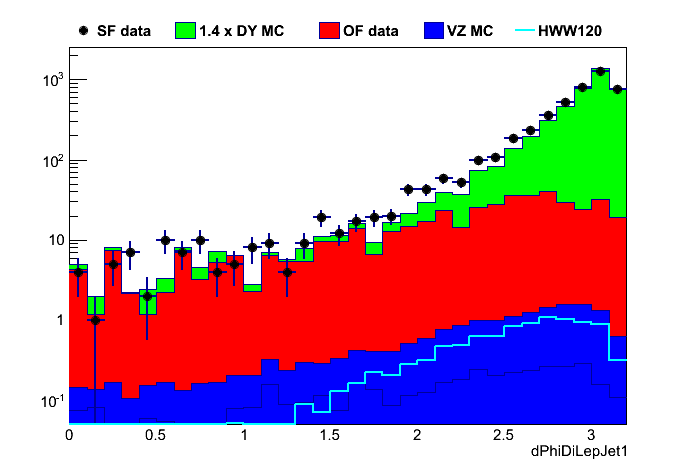
\includegraphics[width=.4\textwidth]{figures/oZMet20ptll45_1j_ll/dPhiDiLepJet1_1j.png}}
\caption{$\Delta\phi$($\Lep\Lep$,j1) distribution in data and MC for 0- and 1-jet bin, where
Z veto $\equiv$ $|$\mll-$m_Z$$|$$>$15~\GeVcc and Z peak $\equiv$ $|$\mll-$m_Z$$|$$<$7.5~\GeVcc.}
\label{fig:dPhiDiLepJet1}
\end{center}
\end{figure}
%%%%%%%%

%%%%%%%%
\begin{figure}[!hbtp]
\begin{center}
\subfigure[Z peak, 0-jet]{\label{subfig:ZpMet20ptll45_0j_ll/dPhiDiLepMET_0j}
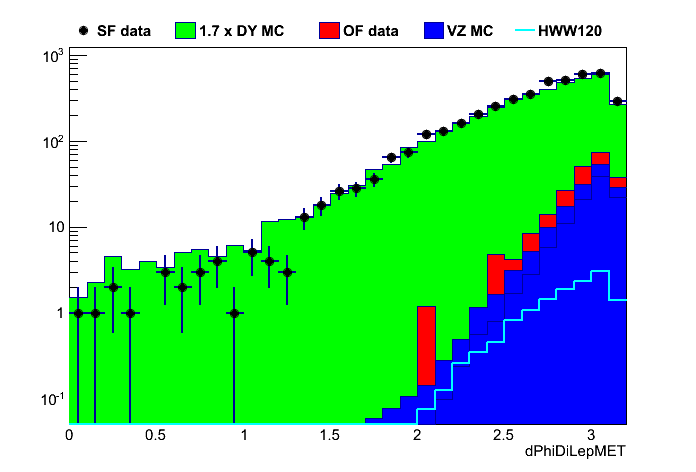
\includegraphics[width=.4\textwidth]{figures/ZpMet20ptll45_0j_ll/dPhiDiLepMET_0j.png}}
\subfigure[Z peak, 1-jet]{\label{subfig:ZpMet20ptll45_1j_ll/dPhiDiLepMET_1j}
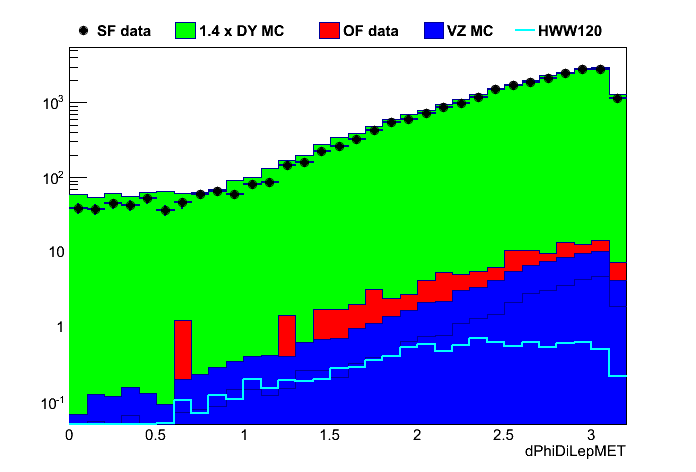
\includegraphics[width=.4\textwidth]{figures/ZpMet20ptll45_1j_ll/dPhiDiLepMET_1j.png}}\\
\subfigure[Z veto, 0-jet]{\label{subfig:oZMet20ptll45_0j_ll/dPhiDiLepMET_0j}
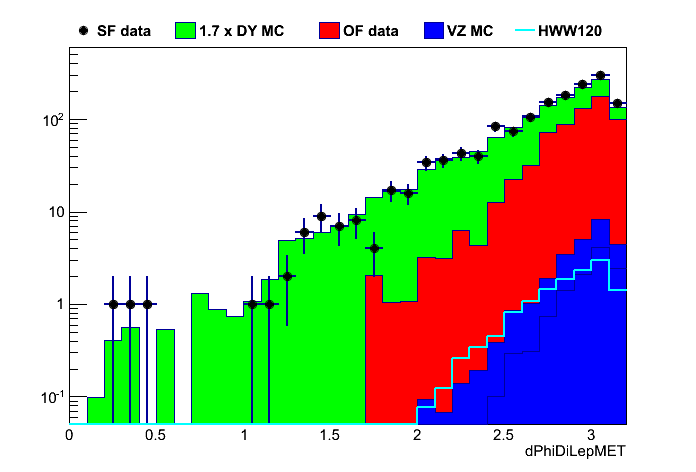
\includegraphics[width=.4\textwidth]{figures/oZMet20ptll45_0j_ll/dPhiDiLepMET_0j.png}}
\subfigure[Z veto, 1-jet]{\label{subfig:oZMet20ptll45_1j_ll/dPhiDiLepMET_1j}
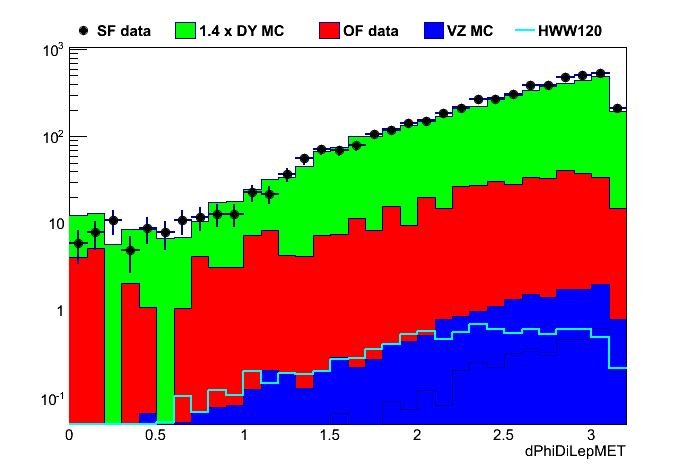
\includegraphics[width=.4\textwidth]{figures/oZMet20ptll45_1j_ll/dPhiDiLepMET_1j.png}}
\caption{$\Delta\phi$($\Lep\Lep$,\met) distribution in data and MC for 0- and 1-jet bin, where
Z veto $\equiv$ $|$\mll-$m_Z$$|$$>$15~\GeVcc and Z peak $\equiv$ $|$\mll-$m_Z$$|$$<$7.5~\GeVcc.}
\label{fig:dPhiDiLepMET}
\end{center}
\end{figure}
%%%%%%%%

%%%%%%%%
\begin{figure}[!hbtp]
\begin{center}
\subfigure[Z peak, 0-jet]{\label{subfig:ZpMet20ptll45_0j_ll/dPhiJet1MET_0j}
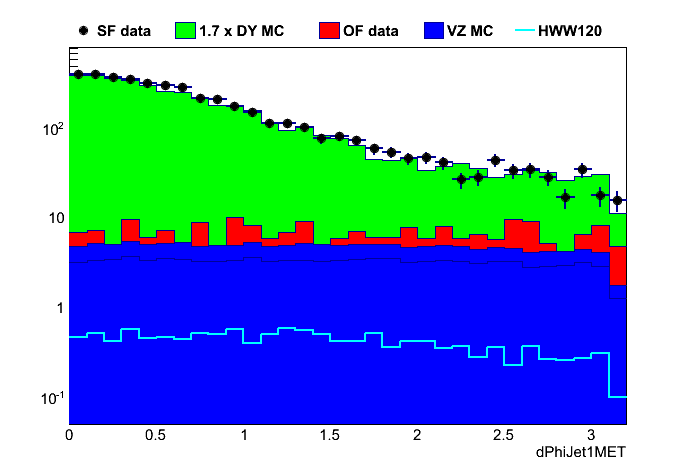
\includegraphics[width=.4\textwidth]{figures/ZpMet20ptll45_0j_ll/dPhiJet1MET_0j.png}}
\subfigure[Z peak, 1-jet]{\label{subfig:ZpMet20ptll45_1j_ll/dPhiJet1MET_1j}
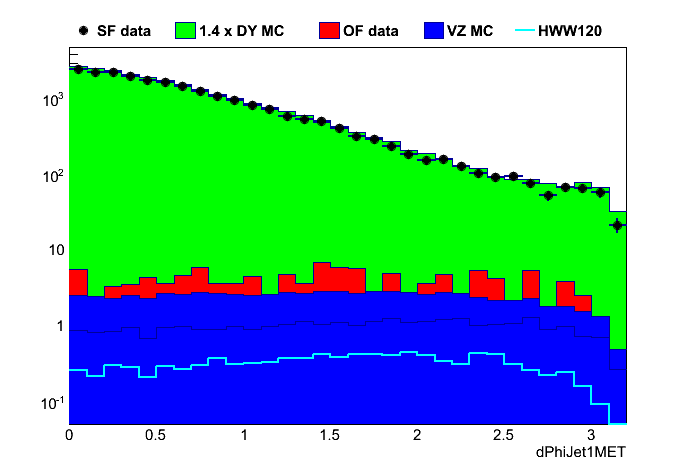
\includegraphics[width=.4\textwidth]{figures/ZpMet20ptll45_1j_ll/dPhiJet1MET_1j.png}}\\
\subfigure[Z veto, 0-jet]{\label{subfig:oZMet20ptll45_0j_ll/dPhiJet1MET_0j}
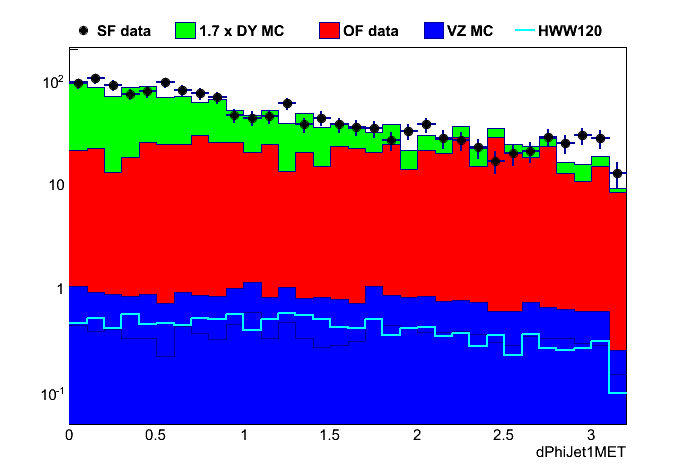
\includegraphics[width=.4\textwidth]{figures/oZMet20ptll45_0j_ll/dPhiJet1MET_0j.png}}
\subfigure[Z veto, 1-jet]{\label{subfig:oZMet20ptll45_1j_ll/dPhiJet1MET_1j}
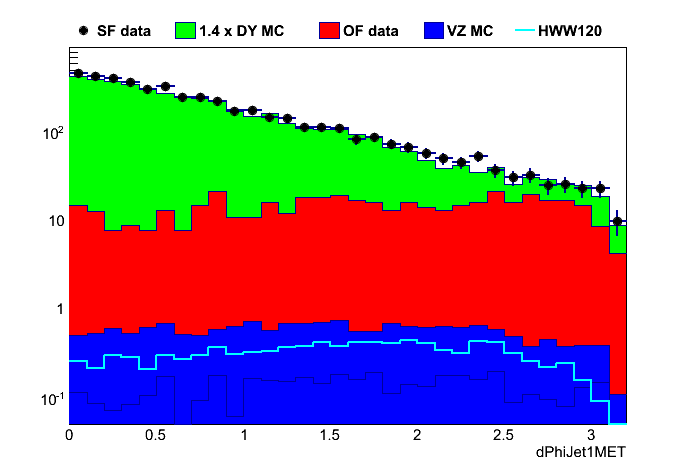
\includegraphics[width=.4\textwidth]{figures/oZMet20ptll45_1j_ll/dPhiJet1MET_1j.png}}
\caption{$\Delta\phi$(j1,\met) distribution in data and MC for 0- and 1-jet bin, where
Z veto $\equiv$ $|$\mll-$m_Z$$|$$>$15~\GeVcc and Z peak $\equiv$ $|$\mll-$m_Z$$|$$<$7.5~\GeVcc.}
\label{fig:dPhiJet1MET}
\end{center}
\end{figure}
%%%%%%%%

%%%%%%%%
\begin{figure}[!hbtp]
\begin{center}
\subfigure[Z peak, 0-jet]{\label{subfig:ZpMet20ptll45_0j_ll/nvtx_0j}
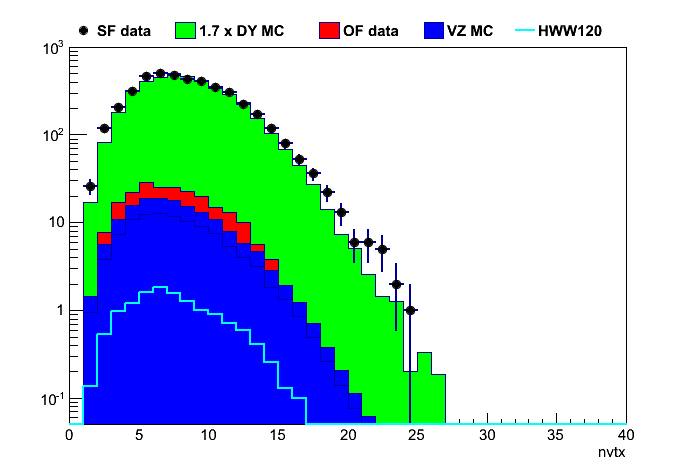
\includegraphics[width=.4\textwidth]{figures/ZpMet20ptll45_0j_ll/nvtx_0j.png}}
\subfigure[Z peak, 1-jet]{\label{subfig:ZpMet20ptll45_1j_ll/nvtx_1j}
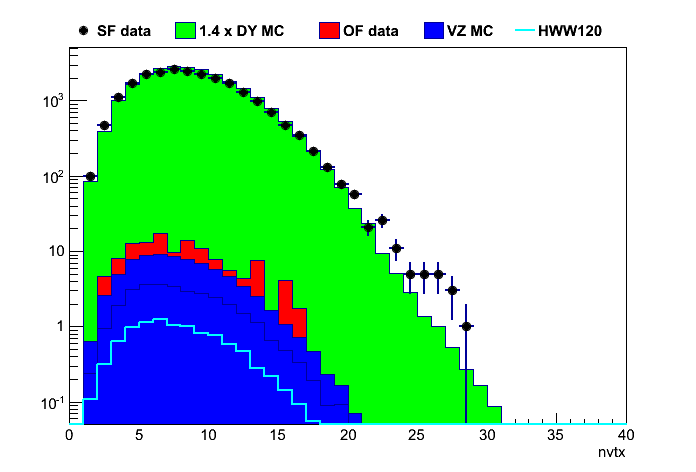
\includegraphics[width=.4\textwidth]{figures/ZpMet20ptll45_1j_ll/nvtx_1j.png}}\\
\subfigure[Z veto, 0-jet]{\label{subfig:oZMet20ptll45_0j_ll/nvtx_0j}
\includegraphics[width=.4\textwidth]{figures/oZMet20ptll45_0j_ll/nvtx_0j.png}}
\subfigure[Z veto, 1-jet]{\label{subfig:oZMet20ptll45_1j_ll/nvtx_1j}
\includegraphics[width=.4\textwidth]{figures/oZMet20ptll45_1j_ll/nvtx_1j.png}}
\caption{Number of vertices distribution in data and MC for 0- and 1-jet bin, where
Z veto $\equiv$ $|$\mll-$m_Z$$|$$>$15~\GeVcc and Z peak $\equiv$ $|$\mll-$m_Z$$|$$<$7.5~\GeVcc.}
\label{fig:nvtx}
\end{center}
\end{figure}
%%%%%%%%

\clearpage

\subsection{Alternative Training On Z Peak Data}
\label{sec:zdatatrain}
It is worth remarking that an alternative training, based on DY events under the Z peak, has been tested. 
Given the approximate description of the fake missing energy in the simulation, we wanted to test whether using real data 
for training could increase the rejection power against DY events.

MVA training on data is a non trivial problem because of background events contaminating the Z peak sample. 
These backgrounds (Top, \W\W\, Wjets, \W\Z, \Z\Z) - negligible in the bulk of the distributions - dominate the tail of \met-related variables 
(top plots in Figures~\ref{fig:pmet}-\ref{fig:mt}) and the MVA should not be trained against non-DY events. 
The solution we found to this problem is to give negative weight to the background events (red and blue area in the plots) and to use a MVA method that can 
properly deal with them in the training (BDTB)~\cite{TMVA2007}. 
The final result, however, is not better than what achieved with the MC training, with a sensitivity improvement in the same range and a slightly worse signal efficiency 
for same DY rejection.

This test has been presented in~\cite{ref:dymvadata}. 

